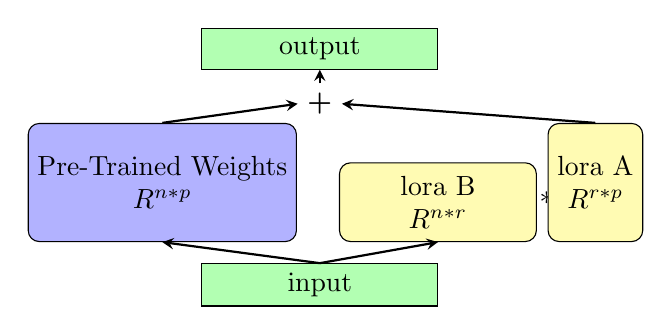
\begin{tikzpicture}[node distance=1.5cm]
% Define block styles
\tikzstyle{weights} = [rectangle,rounded corners, minimum width=2.5cm, minimum height=1.5cm, text centered, draw=black, fill=blue!30]
\tikzstyle{lora_a} = [rectangle,rounded corners, minimum width=1cm, minimum height=1.5cm, text centered, draw=black, fill=yellow!30]
\tikzstyle{lora_b} = [rectangle,rounded corners, minimum width=2.5cm, minimum height=1cm, text centered, draw=black, fill=yellow!30]
\tikzstyle{vector} = [rectangle, minimum width=3cm, minimum height=0.5cm, text centered, draw=black, fill=green!30]
\tikzstyle{arrow} = [thick,->,>=stealth]

% Define nodes
\node (weights) [weights, align=center]{Pre-Trained Weights \\ $\mathbb{R}^{n*p}$};
\node (lora_B) [lora_b, right of=weights,xshift=2cm,yshift=-0.25cm, align=center]{lora B\\ $\mathbb{R}^{n*r}$};
\node (mul) [right of = lora_B,xshift=-0.12cm]{*};
\node (lora_A) [lora_a, right of=lora_B,xshift=0.5cm,yshift=0.25cm, align=center]{lora A\\$\mathbb{R}^{r*p}$};
\node (input) [vector,below of = weights, xshift = 2cm,yshift=+0.2cm]{input};
\node (plus) [above of = weights, xshift = 2cm,yshift=-0.5cm]{\textbf{+}};
\node (output) [vector,above of = plus,yshift=-0.8cm]{output};




% Draw arrows
\draw [arrow] (input.north) -- (weights.south);
\draw [arrow] (input.north) -- (lora_B.south);
\draw [arrow] (weights.north) -- (plus.west);
\draw [arrow] (lora_A.north) -- (plus.east);
\draw [arrow] (plus) -- (output);


\end{tikzpicture}